\documentclass[Lau, binding=0.6cm, oneside]{sapthesis}
\usepackage [italian]{babel}
\usepackage[T1]{fontenc}
\usepackage[utf8]{inputenc}
\usepackage{microtype}
\usepackage{amsmath}
\usepackage{amssymb}
\usepackage{graphicx}
\usepackage{hyperref}
\usepackage{listings}
\usepackage{float}
\usepackage{xurl}
\hypersetup{pdftitle={Collision Avoidance per Robot Mobili},pdfauthor={Davide Albano}}
\linespread{1.5}
\graphicspath{{./img/}}
\lstset{
language=Python,
basicstyle=\footnotesize,
numbers=none,
numberstyle=\footnotesize,
stepnumber=1,
numbersep=5pt,
backgroundcolor=\color{white},
showspaces=false,
showstringspaces=false,
showtabs=false,
frame=single,
tabsize=2,
captionpos=b,
breaklines=true,
breakatwhitespace=false,
escapeinside={\%*}{*)}
}

\title{Collision Avoidance per Robot Mobili}
\author{Davide Albano}
\IDnumber{1708530}
\course{Ingegneria Informatica e Automatica}
\courseorganizer{Facoltà di Ingegneria dell'Informazione, Informatica e Statistica}
\AcademicYear{2020/2021}
\copyyear{2021}
\advisor{Prof. Giorgio Grisetti}
\authoremail{albano.1708530@studenti.uniroma1.it}

\versiondate{ } %queste tre righe non serve che le compili poi quando vai a stampare fai togliere questa parte perchè non si può cancellare sennò non parte il file
\begin{document}
\maketitle
\begin{abstract}
L'obiettivo di questo lavoro è la realizzazione di un sistema che permetta a un robot di muoversi all'interno di un ambiente evitando eventuali ostacoli.
Il robot preso in considerazione non conosce l'ambiente in cui dovrà muoversi e può quindi basarsi soltanto sulle rilevazioni fatte tramite un laser scanner.

Per l'implementazione è stato usato ROS (Robot Operating System), un framework open source pensato per gestire le operazioni e le comunicazioni dei vari nodi di un robot.
Per la simulazione è stato usato il pacchetto stage\_ros, mentre per la visualizzazione delle informazioni dei vari sensori e della traiettoria calcolata dal robot è stato usato il tool RVIZ.

Data l'assenza di informazioni iniziali riguardo alla mappa è stata necessario scegliere un algoritmo di local motion control.
In particolare, è stato scelto il metodo dell'Artificial Potential Field, che è spesso usato per la sua semplicità sia dal punto di vista dello sviluppo sia dal punto di vista computazionale.
\end{abstract}
\tableofcontents

\chapter{Introduzione}
\section{Formulazione problema}
Lo sviluppo di algoritmi di navigazione autonoma per robot mobili deve affrontare due problematiche quindi si suddivide in due parti \cite{fonte1}:
\begin{description}
	\item[global path planning] Algoritmi che utilizzano le informazioni che si hanno sulla mappa per trovare il percorso più breve per andare dal punto di partenza all'obiettivo.
	\item[local motion control] Algoritmi che permettono al robot di calcolare in tempo reale una traiettoria in grado di evitare gli ostacoli incontrati durante la navigazione.
\end{description}

La necessità degli algoritmi di local motion control nasce nel momento in cui le informazioni sulla mappa sono incomplete o possono essere soggette a cambiamenti, come avviene in ambienti dinamici con ostacoli in movimento.
Tutti gli algoritmi di local motion control hanno quindi il fine di condurre il robot verso un obiettivo valutando in ogni istante di tempo il percorso più sicuro.
A differenza degli algoritmi di global path planning non hanno una parte di pre-pianificazione ma si basano soltanto sulla pianificazione real-time.

\section{Importanza della Collision Avoidance}
In un mondo che tende sempre di più all'automazione, il problema della Collision Avoidance diventa sempre di maggiore rilievo.
Gli utilizzi principali di questo tipo di algoritmi si possono trovare nel settore dei trasporti e nell'Industry 4.0.

\subsection{Settore dei trasporti}
All'interno del settore dei trasporti sono in corso numerosi studi dal punto di vista dei trasporti via terra.
In particolare, sono molte le aziende automobilistiche (tra cui spiccano principalmente Tesla, Waymo e Pony.ai) che stanno investendo nello sviluppo di sistemi di guida autonoma.
Questi sistemi devono tra le altre cose essere in grado di reagire a tutti gli imprevisti che si possono normalmente incontrare durante la guida, compresa ovviamente la presenza improvvisa di ostacoli lungo il tragitto.

Anche se le auto a guida totalmente autonoma sono ancora in fase di test, alcune funzioni di Collision Avoidance sono già realizzate dalla maggior parte delle case automobilistiche; tra queste funzioni troviamo \cite{fonte8}:
\begin{description}
	\item[Adaptive Cruise Control] Questo sistema usa radar e laser per adattare la velocità in modo da mantenere la giusta distanza dal veicolo che sta davanti.
	\item[Automatic Emergency Braking (AEB)] In questo caso vengono attivati i freni per evitare una collisione o per ridurre la velocità di impatto.
	\item[Rear Automatic Emergency Braking] I freni vengono attivati per evitare collisioni quando il veicolo sta indietreggiando.
	\item[Electronic Stability Control (ESC)] Applica automaticamente i freni per aiutare a guidare l'auto durante una perdita di trazione. Un computer di bordo monitora vari sensori per determinare quali ruote frenare e quali accelerare.
	\item[Parking Assist] I feedback delle telecamere e dei sensori vengono combinati per consentire al veicolo di sterzare in un parcheggio mentre il conducente controlla la velocità.
\end{description} 

Anche per gli spostamenti via mare e via aria sono in corso studi riguardanti la navigazione autonoma, con particolare interesse per i droni sottomarini (UUV) e aerei (UAV).

\begin{figure}[H]
    \centering
    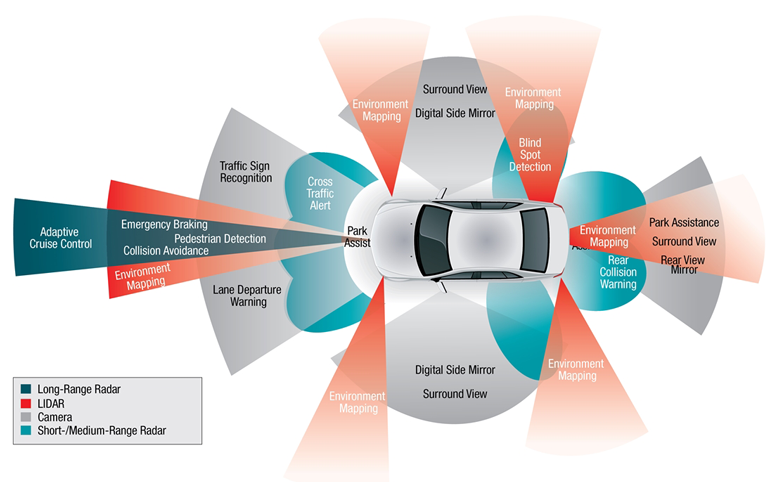
\includegraphics[width=12.5cm]{driverless_car.png}
    \caption{In questa immagine si possono vedere i sensori che sono necessari per poter avere un'auto a guida completamente autonoma.}
    \label{fig:driverless_car}
\end{figure}

\subsection{Industry 4.0}
Per quanto riguarda il settore industriale, sempre più aziende stanno passando all'Industry 4.0, che prevede una automazione avanzata all'interno degli impianti produttivi.
In fabbriche dove più robot mobili lavorano anche a contatto con gli operatori diventa essenziale che essi riconoscano la presenza di altri robot e soprattutto di umani, per garantire una maggiore sicurezza.
In questo caso entrano in campo i sistemi di Collision Avoidance, perché anche se la mappa generale può essere ben nota, gli ostacoli possono muoversi liberamente all'interno dell'area.

Ne è un esempio il sistema anticollisione SmartDect, un dispositivo sviluppato dall'azienda italiana Elettric80 che mira a ridurre notevolmente il rischio di collisioni tra Automated Guided Vehicles (AGVs) e i dipendenti \cite{fonte9}.
Questo sistema prevede un dispositivo indossabile con tecnologia Ultra-Wide Band (UWB) che sarà indossato dagli operatori o posizionato sui veicoli a guida manuale.
Questo dispositivo comunica in tempo reale la sua posizione ai veicoli a guida automatica, facilitando in questo modo la prevenzione della collisione.
Questo sistema è dotato inoltre di un'altra funzione: infatti nelle situazioni di rischio, oltre a rallentare, l'AGV invierà un segnale al dispositivo, il quale inizierà a vibrare o lampeggiare per avvertire l'operatore \cite{fonte10}.

\begin{figure}[H]
    \centering
    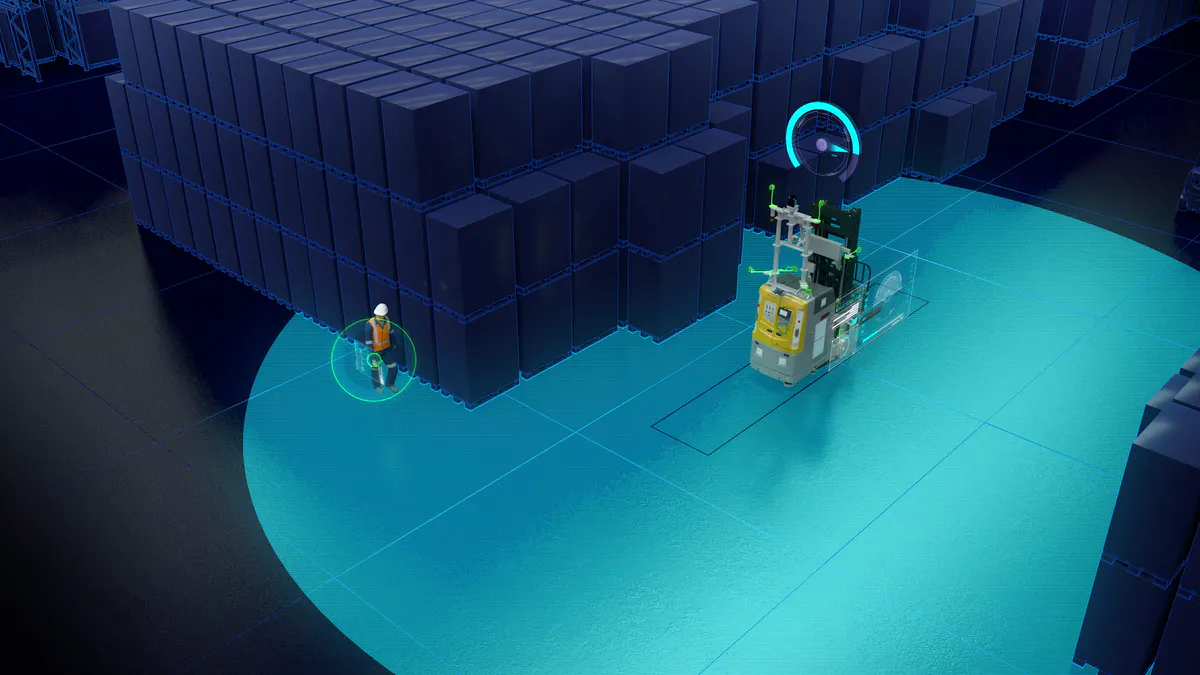
\includegraphics[width=12.5cm]{smart_dect.png}
    \caption{Questa immagine mostra il funzionamento della comunicazione tra il dispositivo SmartDect e un veicolo a guida autonoma che si trova nei paraggi.}
    \label{fig:smart_dect}
\end{figure}

\section{Obiettivo di questo progetto}
L'obiettivo di questo progetto è quello di sviluppare un sistema di Collision Avoidance basato su un laser scanner con le seguenti caratteristiche:
\begin{description}
	\item[Input] Il sistema prende in input lo scan del laser e un comando di velocità
	\item[Output] Il sistema produce un comando di velocità che previene la collisione con gli oggetti rilevati nel contorno, deflettendo la traiettoria del robot verso uno spazio libero da ostacoli.
\end{description}
Quindi, a differenza della definizione classica del problema, nel caso analizzato non avremo un obiettivo da raggiungere ma una velocità iniziale del robot, su cui si andrà a intervenire affinché il robot non vada ad urtare qualcosa.

\chapter{Strumenti necessari e teoria}
\section{ROS}
\subsection{Caratteristiche principali}
ROS (Robot Operating System) è un framework open source utilizzato per lo sviluppo di applicazioni per la robotica.
Mette infatti a disposizione strumenti e librerie utili per aiutare gli sviluppatori software nella realizzazione di applicazioni robotiche a partire dalla scrittura fino all’esecuzione e al debugging del codice.

ROS presenta inoltre alcune caratteristiche di un sistema operativo (gestione di processi, di pacchetti e delle loro dipendenze e astrazione di dispositivi hardware a basso livello) e di un middleware perché permette la comunicazione tra processi/macchine diverse.

Infine, costituisce un’architettura distribuita in cui è possibile gestire in maniera asincrona un insieme di moduli software che possono essere scritti in vari linguaggi, tra cui C++ e Python.

Uno dei principali punti di forza di ROS è la sua modularità, che gli permette di essere compatibile con robot che hanno caratteristiche molto diverse tra loro.
La modularità rende inoltre più facile riutilizzare il codice e permette di integrare ROS con altri framework.

ROS include anche alcuni tool che permettono di simulare hardware e di salvare i dati ottenuti dai vari sensori per poi analizzarli.

Il software viene organizzato in packages. Ogni package può contenere più eseguibili, chiamati nodi.
I nodi possono comunicare tra loro in due modi, tramite il meccanismo Publisher/Subscriber oppure tramite il meccanismo dei Services.

ROS è strutturato intorno ad un nodo master che permette ai vari nodi di essere a conoscenza della presenza di altri nodi e di comunicare.
Il master è un nodo unico all’interno dell’architettura di ROS e si occupa di assegnare un nome a ogni nodo connesso al sistema e di registrarlo eventualmente come Publisher, Subscriber o Service Provider.
I vari nodi usano una libreria (ROS client library) per poter usufruire delle funzionalità di ROS, attraverso linguaggio C++ (roscpp) o Python (rospy).
Al nodo master viene assegnato un well-known XML-RPC URI in modo che qualsiasi nodo creato sia sempre in grado di comunicare con esso \cite{fonte3}.

\subsection{Publisher/Subscriber}
È uno dei due meccanismi usati dai vari nodi ROS per comunicare, ed è una modalità di comunicazione asincrona.
La scrittura di un messaggio avviene su un topic da parte dei nodi di tipo Publisher e tutti i nodi di tipo Subscriber che desiderano ricevere tale messaggio possono iscriversi a quel topic.
Per uno stesso topic possono esserci più Publisher e più Subscriber.

Il messaggio è una struttura dati con diversi campi che possono essere di tipi diversi (sono supportati tutti i tipi standard primitivi come integer, float, double, boolean e string).
All’interno di un topic è possibile scrivere o leggere solo un tipo di messaggio.
La definizione dei vari tipi di messaggi viene memorizzata in file .msg.

Nello sviluppo successivamente illustrato questo meccanismo di comunicazione è stato utilizzato per leggere le informazioni inviate dal laser scanner e la velocità in input e per scrivere in output la velocità ricalcolata in base agli ostacoli presenti.
Sono stati usati i messaggi anche per pubblicare su un topic che è stato poi importato in RVIZ per visualizzare le informazioni sulla forza calcolata.

\subsection{Services}
Questa modalità di comunicazione tra nodi è invece sincrona e usa la semantica Request/Response.
Un nodo invia una richiesta a tutti i nodi che forniscono un determinato servizio.
Da questi nodi riceverà una risposta.

La struttura dati usata dai servizi è simile a quella dei messaggi, ma ha una sezione per la Request e una per la Response, separate da una riga contenente i caratteri "\lstinline{---}".
La definizione dei vari tipi di servizi viene memorizzata in file .srv.

Nel caso qui presentato questa modalità è stata utilizzata per fornire il risultato dei calcoli effettuati sugli ostacoli circostanti al nodo che si occuperà poi di determinare la velocità e la direzione di output.

\subsection{stage\_ros}
Questo package è stato utilizzato per la simulazione del robot e dell'ambiente circostante, compresi i vari ostacoli:

\begin{figure}[H]
    \centering
    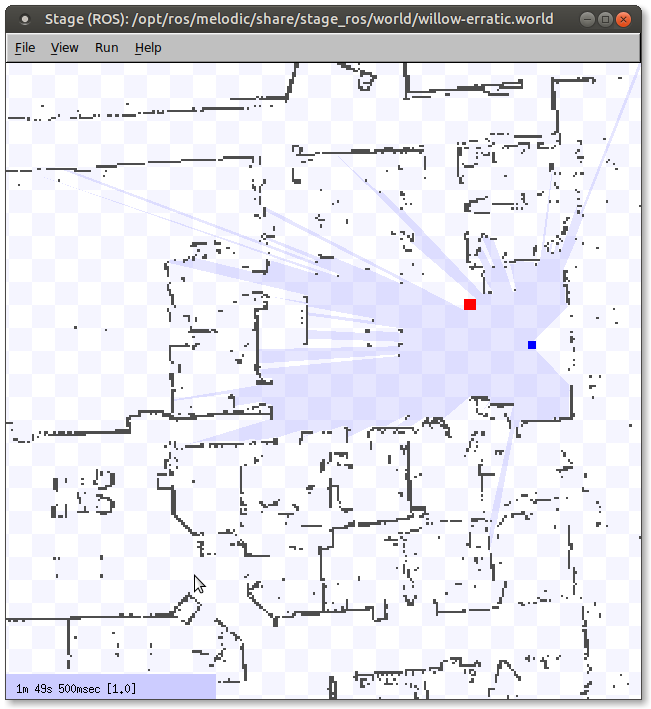
\includegraphics[width=11cm]{stage_ros.png}
    \caption{Schermata di partenza di stage\_ros, in cui si possono vedere il robot (il quadrato blu), il raggio d'azione dello scanner (l'area blu chiaro), gli ostacoli (i tratti grigi) e l'obiettivo (il quadrato rosso).}
    \label{fig:stage_ros}
\end{figure}

\subsection{RVIZ}
RVIZ è stato molto utile per visualizzare in tempo reale le informazioni presenti sui vari topic, come ad esempio la direzione del robot o i rilevamenti effettuati dallo scanner:

\begin{figure}[H]
    \centering
    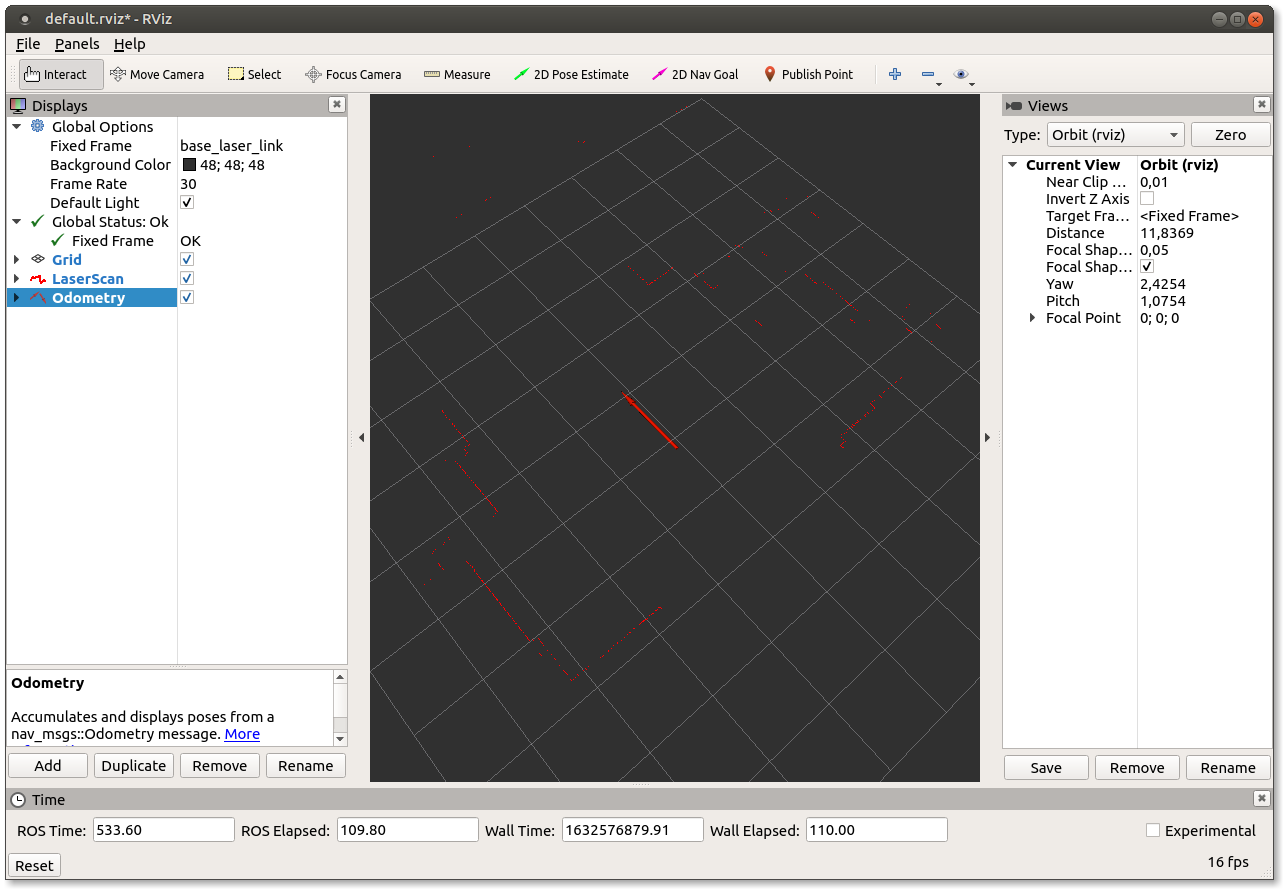
\includegraphics[width=13cm]{rviz.png}
    \caption{Schermata di RVIZ in cui sono state caricate le informazioni dello scanner (i tratti rossi) e della direzione del robot (la freccia rossa)}
    \label{fig:rviz}
\end{figure}

\subsection{teleop\_twist\_keyboard}
Questo tool fornito da ROS permette di inviare dei comandi di movimento su uno specifico topic (di default \textbf{cmd\_vel}) utilizzando alcuni tasti:
\begin{figure}[H]
    \centering
    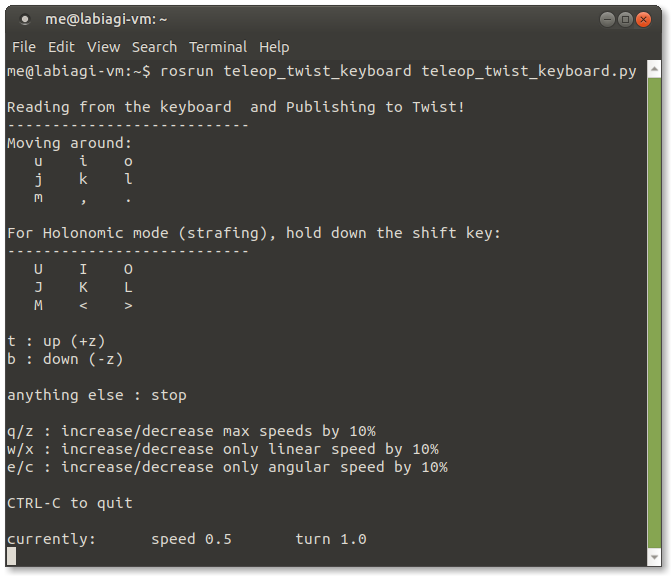
\includegraphics[width=13cm]{teleop.png}
    \caption{Dopo aver lanciato il comando per far partire \textbf{teleop\_twist\_keyboard} il programma ci mostra una legenda dei tasti da cliccare per mandare al robot determinati comandi di movimento.}
    \label{fig:teleop}
\end{figure}
È stato utilizzato per effettuare dei test manuali sull'algoritmo.

\section{Artificial Potential Field}
\subsection{Teoria}
Per quanto riguarda il local motion control, ci sono vari approcci ed algoritmi che possono essere utilizzati, come ad esempio il Vector Field Histogram, il Dynamic Window Approach e l'Artificial Potential Field \cite{fonte1}.
Quest'ultimo metodo è stato scelto per la realizzazione del progetto.

Il metodo dell'Artificial Potential Field si basa sulla seguente idea: l'obiettivo del robot si comporta come una forza attrattiva, mentre gli ostacoli si comportano come forze repulsive.
Il potenziale totale $U$ sarà la somma delle varie forze attrattive e repulsive e il gradiente negativo $-\nabla U(q)$ indicherà la traiettoria più sicura.

Per quanto riguarda le forze attrattive si combinano due profili di attrazione in base alla distanza del robot dall'obiettivo $\boldsymbol{q}_{g}$: conico quando il robot è lontano, paraboidale quando è vicino.
In questo modo la formula per il calcolo della campo attrattivo diventa:
\newline
$$
U_{a}(\boldsymbol{q})=\left\{\begin{array}{cll}
\frac{1}{2} k_{a}\|\boldsymbol{e}(\boldsymbol{q})\|^{2} & \text { if } & \|\boldsymbol{e}(\boldsymbol{q})\| \leq \rho \\
k_{b}\|\boldsymbol{e}(\boldsymbol{q})\| & \text { if } & \|e(\boldsymbol{q})\|>\rho
\end{array}\right.
$$
\newline
dove $\boldsymbol{e}=\boldsymbol{q}_{g}-\boldsymbol{q}$, $k_{a}>0$ e $k_{b}>0$.
Per la continuità della funzione è necessario inoltre che:
$$
k_{a} \boldsymbol{e}(\boldsymbol{q})=k_{b} \frac{\boldsymbol{e}(\boldsymbol{q})}{\|\boldsymbol{e}(\boldsymbol{q})\|} \quad \text { for } \quad\|\boldsymbol{e}(\boldsymbol{q})\|=\rho
$$
\newline
e quindi $k_{b}=\rho k_{a}$.

Per quanto riguarda invece il campo repulsivo, la formula è la seguente:
\newline
$$
U_{r, i}(\boldsymbol{q})=\left\{\begin{array}{ll}
\frac{k_{r, i}}{\gamma}\left(\frac{1}{\eta_{i}(\boldsymbol{q})}-\frac{1}{\eta_{0, i}}\right)^{\gamma} & \text { if } \eta_{i}(\boldsymbol{q}) \leq \eta_{0, i} \\
0 & \text { if } \eta_{i}(\boldsymbol{q})>\eta_{0, i}
\end{array}\right.
$$
\newline
dove $k_{r, i}>0$ e $\gamma=2,3, \ldots$; $\eta_{0, i}$ è il raggio di influenza, mentre $\eta_{i}(\boldsymbol{q})$ è il margine ed è calcolato come segue:
$$
\eta_{i}(\boldsymbol{q})=\min _{\boldsymbol{q}^{\prime} \in \mathcal{C O}_{i}}\left\|\boldsymbol{q}-\boldsymbol{q}^{\prime}\right\|
$$
\newline
dove $\mathcal{C O}_{i}$ è la obstacle region.

Otteniamo così una somma dei campi totali:
$$
U_{t}(\boldsymbol{q})=U_{a}(\boldsymbol{q})+U_{r}(\boldsymbol{q})
$$
da cui possiamo ricavare la formula della forza totale:
$$
\boldsymbol{f}_{t}(\boldsymbol{q})=-\nabla U_{t}(\boldsymbol{q})=\boldsymbol{f}_{a}(\boldsymbol{q})+\sum_{i=1}^{p} \boldsymbol{f}_{r, i}(\boldsymbol{q})
$$
\cite{fonte2}

\subsection{Applicazione per i robot su ruote}
Essendo soggetti a determinati vincoli di movimento, nel caso dei robot su ruote non è possibile applicare direttamente la forza risultante appena calcolata.
Partendo da una forza artificiale $\boldsymbol{f}_{t}=\left(\begin{array}{lll}f_{t, x} & f_{t, y} & f_{t, \theta}\end{array}\right)^{T}$ possiamo tuttavia ottenere:

$$
\begin{array}{l}
v=f_{t, x} \cos \theta+f_{t, y} \sin \theta \\
\omega=f_{t, \theta}
\end{array}
$$
dove $\theta$ è l'angolo formato tra l'asse sagittale del robot e l'asse x del sistema di riferimento \cite{fonte4}, mentre $f_{t, \theta}$ può essere calcolato nel seguente modo \cite{fonte2}:

$$
f_{t, \theta}=k_{\theta}\left(\operatorname{atan} 2\left(f_{t, y}, f_{t, x}\right)-\theta\right)
$$

\chapter{Descrizione del progetto}
\section{Sistema di riferimento}
Poiché nel caso in esame è presente un solo robot mobile e gli ostacoli sono tutti fissi, è stato possibile scegliere come sistema di riferimento il sistema di riferimento mobile del robot.
Questo ha portato a una semplificazione delle formule.
Infatti in questo modo la posizione del robot è sempre $\left(x, y\right)=(0,0)$, mentre l'angolo $\theta$ definito nel capitolo precedente è sempre 0.

Le formule prima presentate diventano quindi:
$$
\begin{array}{l}
v=\left\|\left(f_{t, x}, f_{t, y}\right)\right\| \\
\omega=\operatorname{atan} 2\left(f_{t, y}, f_{t, x}\right)
\end{array}
$$
Infatti, tramite $\omega$ facciamo ruotare il robot nella direzione della forza risultante, e poi lo facciamo muovere linearmente impostando $v$ uguale al modulo della forza.

\section{Nodi}
Per questo progetto sono stati sviluppati tre nodi ROS:
\begin{description}
	\item[twist\_gnerator] Questo nodo si occupa di simulare una serie di comandi di velocità in input.
	\item[obstacle\_detection] Questo nodo si occupa di analizzare le informazioni provenienti dallo scanner e memorizzare i calcoli effettuati su tali informazioni, per poi fornirli tramite un servizio.
	\item[cmd\_vel\_controller] Questo nodo si occupa di intercettare i comandi di velocità in input e calcolare la nuova traiettoria basandosi sulle informazioni ricevute da obstacle\_detection.
\end{description}

\subsection{twist\_generator}
\begin{lstlisting}
#! /usr/bin/env python

import rospy
from geometry_msgs.msg import Twist
from random import random

class twistGenerator:
    def __init__(self):
        self.pub = rospy.Publisher('/cmd_vel_input', Twist, queue_size=10)
        self.move()
    
    def move(self):
        vel_msg = Twist()
        vel_msg.linear.x = 0
        vel_msg.linear.y = 0
        vel_msg.linear.z = 0
        vel_msg.angular.x = 0
        vel_msg.angular.y = 0
        vel_msg.angular.z = -5 + random() * 10
        self.pub.publish(vel_msg)
        vel_msg.angular.z = 0
        while not rospy.is_shutdown():
            vel_msg.linear.x = random() * 10
            self.pub.publish(vel_msg)


def main():
    rospy.init_node('twist_generator', anonymous=True)
    twist = twistGenerator()
    try:
        rospy.spin()
    except KeyboardInterrupt:
        print("Shutting down")

if __name__ == '__main__':
    main()
\end{lstlisting}

Per poter scrivere sul topic di input della velocità \textbf{cmd\_vel\_input}, questo nodo deve innanzitutto registrarsi come Publisher su quel topic:

\begin{lstlisting}
    self.pub = rospy.Publisher('/cmd_vel_input', Twist, queue_size=10)
\end{lstlisting}

Il nodo andrà quindi a chiamare la funzione \textbf{move}, che scriverà sul topic un primo messaggio con una velocità angolare casuale e poi inizierà a inviare una serie di messaggi con velocità lineare casuale:

\begin{lstlisting}
def move(self):
    vel_msg = Twist()
    ...
    vel_msg.angular.z = -5 + random() * 10
    self.pub.publish(vel_msg)
    vel_msg.angular.z = 0
    while not rospy.is_shutdown():
        vel_msg.linear.x = random() * 10
        self.pub.publish(vel_msg)
\end{lstlisting}
In questo modo il robot partirà con una direzione iniziale sempre diversa e poi continuerà ad andare avanti con velocità scelte in modo randomico.

\subsection{obstacle\_detection}
\begin{lstlisting}
#! /usr/bin/env python

import rospy
from sensor_msgs.msg import LaserScan
import math
from collision_avoidance.srv import Force, ForceResponse
from visualization_msgs.msg import Marker
from tf.transformations import quaternion_from_euler

class obstacleDetection:
    def __init__(self):
        self.sub = rospy.Subscriber('/base_scan', LaserScan, self.callback)
        self.pub = rospy.Publisher('marker', Marker, queue_size=10)
        self.srv = rospy.Service('force_service', Force, self.force_service)
        self.force = ForceResponse(0, 0)

    def callback(self, msg):
        self.force = ForceResponse(0, 0)
        for i, val in enumerate(msg.ranges, start=0):
            if val >= 1.25:
                continue
            magnitude = 1 / val
            temp_angle = msg.angle_min + (i * msg.angle_increment)
            x = magnitude * math.cos(temp_angle)
            y = magnitude * math.sin(temp_angle)
            angle = math.atan2(-y, -x)
            force = ForceResponse(magnitude, angle)
            self.set_net_force(force)
        self.show_force()
    
    def set_net_force(self, force):
        x1 = self.force.magnitude * math.cos(self.force.angle)
        y1 = self.force.magnitude * math.sin(self.force.angle)
        x2 = force.magnitude * math.cos(force.angle)
        y2 = force.magnitude * math.sin(force.angle)
        x_total = x1 + x2
        y_total = y1 + y2
        total_magnitude = math.sqrt(x_total ** 2 +  y_total ** 2)
        total_angle = math.atan2(y_total, x_total)
        self.force = ForceResponse(total_magnitude, total_angle)

    def show_force(self):
        self.marker = Marker()
        self.marker.header.frame_id = '/base_link'
        self.marker.header.stamp = rospy.get_rostime()
        self.marker.ns = 'robot'
        self.marker.id = 0
        self.marker.type = 0
        self.marker.action = 0

        self.marker.pose.position.x = 0
        self.marker.pose.position.y = 0
        self.marker.pose.position.z = 0

        q = quaternion_from_euler(0, 0, self.force.angle)
        self.marker.pose.orientation.x = q[0]
        self.marker.pose.orientation.y = q[1]
        self.marker.pose.orientation.z = q[2]
        self.marker.pose.orientation.w = q[3]

        self.marker.scale.x = self.force.magnitude
        self.marker.scale.y = 0.05
        self.marker.scale.z = 0.05

        self.marker.color.r = 0.0
        self.marker.color.g = 1.0
        self.marker.color.b = 0.0
        self.marker.color.a = 1.0

        self.marker.lifetime = rospy.Duration(0)

        self.pub.publish(self.marker)

    def force_service(self, request):
        return self.force

def main():
    rospy.init_node('obstacle_detection', anonymous=True)
    od = obstacleDetection()
    try:
        rospy.spin()
    except KeyboardInterrupt:
        print("Shutting down")

if __name__ == '__main__':
    main()
\end{lstlisting}

La parte principale di questo nodo è l'analisi delle informazioni che lo scanner scrive nel topic \textbf{base\_scan}.
Per poter leggere queste informazioni il nodo come prima cosa si iscrive al topic, specificando la callback che deve essere chiamata appena viene scritto un nuovo messaggio:

\begin{lstlisting}
    self.sub = rospy.Subscriber('/base_scan', LaserScan, self.callback)
\end{lstlisting}

Questo nodo dovrà inoltre registrarsi come Publisher sul topic \textbf{marker}, dove scriverà le informazioni calcolate, che verranno poi lette da RVIZ:

\begin{lstlisting}
    self.pub = rospy.Publisher('marker', Marker, queue_size=10)
\end{lstlisting}

Dovrà infine registrarsi come provider del servizio \textbf{force\_service} e inizializzare la variabile \textbf{force}.
La forza risultante agente sul robot viene infatti calcolata da questo nodo, salvata nella variabile \textbf{force} e poi fornita a qualunque nodo la richieda:

\begin{lstlisting}
    self.srv = rospy.Service('force_service', Force, self.force_service)
    self.force = ForceResponse(0, 0)
\end{lstlisting}

\begin{lstlisting}
def force_service(self, request):
    return self.force
\end{lstlisting}

Ogni volta che lo scanner inserirà una nuova rilevazione sotto forma di messaggio nel topic \textbf{base\_scan}, verrà quindi chiamata la callback, che filtrerà i dati rilevati in base a un parametro di soglia (in questo caso \lstinline{1.25}), ne calcolerà l'equivalente forza repulsiva e infine invocherà per ogni valore calcolato la funzione \textbf{set\_net\_force}:

\begin{lstlisting}
def callback(self, msg):
    self.force = ForceResponse(0, 0)
    for i, val in enumerate(msg.ranges, start=0):
        if val >= 1.25:
            continue
        magnitude = 1 / val
        temp_angle = msg.angle_min + (i * msg.angle_increment)
        x = magnitude * math.cos(temp_angle)
        y = magnitude * math.sin(temp_angle)
        angle = math.atan2(-y, -x)
        force = ForceResponse(magnitude, angle)
        self.set_net_force(force)
    self.show_force()
\end{lstlisting}

La funzione \textbf{set\_net\_force} si occuperà quindi di calcolare progressivamente la risultante delle varie forze analizzate dalla callback e di salvare il risultato nella variabile \textbf{force}:

\begin{lstlisting}
def set_net_force(self, force):
    x1 = self.force.magnitude * math.cos(self.force.angle)
    y1 = self.force.magnitude * math.sin(self.force.angle)
    x2 = force.magnitude * math.cos(force.angle)
    y2 = force.magnitude * math.sin(force.angle)
    x_total = x1 + x2
    y_total = y1 + y2
    total_magnitude = math.sqrt(x_total ** 2 +  y_total ** 2)
    total_angle = math.atan2(y_total, x_total)
    self.force = ForceResponse(total_magnitude, total_angle)
\end{lstlisting}

Infine, all'interno della funzione \textbf{show\_force}, viene creato un oggetto di tipo \textbf{Marker}, che verrà pubblicato sul topic \textbf{marker} per poi essere importato in RVIZ.
Questo oggetto rappresenta la forza risultante tramite una freccia (\lstinline{self.marker.type = 0}).
Viene quindi usato l'angolo della forza per calcolare l'orientamento della freccia e il modulo per calcolarne la lunghezza.
Infine viene scelto il colore della freccia (verde in questo caso) e viene pubblicato il marker sul topic:

\begin{lstlisting}
def show_force(self):
    self.marker = Marker()
    ...
    self.marker.type = 0
    ...

    q = quaternion_from_euler(0, 0, self.force.angle)
    self.marker.pose.orientation.x = q[0]
    self.marker.pose.orientation.y = q[1]
    self.marker.pose.orientation.z = q[2]
    self.marker.pose.orientation.w = q[3]

    self.marker.scale.x = self.force.magnitude
    ...

    self.marker.color.r = 0.0
    self.marker.color.g = 1.0
    self.marker.color.b = 0.0
    self.marker.color.a = 1.0

    ...

    self.pub.publish(self.marker)
\end{lstlisting}

\subsection{cmd\_vel\_controller}
\begin{lstlisting}
#! /usr/bin/env python

import rospy
from geometry_msgs.msg import Twist
from collision_avoidance.srv import Force

class cmdVelController:
    def __init__(self):
        self.pub = rospy.Subscriber('/cmd_vel_input', Twist, self.callback)
        self.pub = rospy.Publisher('/cmd_vel', Twist, queue_size=10)
    
    def callback(self, msg):
        if msg.linear.x == 0:
            self.pub.publish(msg)
            return
        rospy.wait_for_service('force_service')
        try:
            force_service = rospy.ServiceProxy('force_service', Force)
            force = force_service()
            vel_msg = Twist()
            x_linear = msg.linear.x + force.magnitude
            vel_msg.linear.x = x_linear if x_linear < 0.75 else 0.75
            vel_msg.linear.y = 0
            vel_msg.linear.z = 0
            vel_msg.angular.x = 0
            vel_msg.angular.y = 0
            vel_msg.angular.z = msg.angular.z + force.angle
            self.pub.publish(vel_msg)
        except rospy.ServiceException as e:
            print('Service call failed: %s' %e)


def main():
    rospy.init_node('cmd_vel_controller', anonymous=True)
    cmd = cmdVelController()
    try:
        rospy.spin()
    except KeyboardInterrupt:
        print("Shutting down")

if __name__ == '__main__':
    main()
\end{lstlisting}

Questo nodo si occupa di leggere la velocità di input e di scrivere in output la velocità ricalcolata in base alla forza repulsiva risultante.
Per fare ciò deve registrarsi come Subscriber al topic \textbf{cmd\_vel\_input} e come Publisher al topic \textbf{cmd\_vel}:

\begin{lstlisting}
    self.pub = rospy.Subscriber('/cmd_vel_input', Twist, self.callback)
    self.pub = rospy.Publisher('/cmd_vel', Twist, queue_size=10)
\end{lstlisting}

Nella funzione di callback chiamerà quindi il servizio \textbf{force\_service} che gli fornirà il valore corrente della forza repulsiva risultante.
Con il risultato della chiamata a questo servizio popolerà i valori della velocità lineare sull'asse x e di quella angolare sull'asse z.
Infine invierà il messaggio sul topic \textbf{cmd\_vel}, che corrisponde al topic di input del robot:

\begin{lstlisting}
def callback(self, msg):
    ...
    rospy.wait_for_service('force_service')
    try:
        force_service = rospy.ServiceProxy('force_service', Force)
        force = force_service()
        vel_msg = Twist()
        x_linear = msg.linear.x + force.magnitude
        vel_msg.linear.x = x_linear if x_linear < 0.75 else 0.75
        ...
        vel_msg.angular.z = msg.angular.z + force.angle
        self.pub.publish(vel_msg)
    except rospy.ServiceException as e:
        print('Service call failed: %s' %e)
\end{lstlisting}

\section{Messaggi}
\subsection{geometry\_msgs/Twist.msg}
La definizione del tipo Twist.msg è presente nella libreria fornita da ROS, ed è la seguente \cite{fonte5}:
\begin{lstlisting}
# This expresses velocity in free space broken into its linear and angular parts.

Vector3  linear
Vector3  angular
\end{lstlisting}
I messaggi di tipo Twist sono quelli che sono usati sui topic \textbf{cmd\_vel\_input} e \textbf{cmd\_vel}.
Ogni variabile di tipo Vector3 è composta da 3 componenti, che in questo caso corrispondono alle componenti  $(x, y, z)$ delle velocità lineare e angolare.

\subsection{sensor\_msgs/LaserScan.msg}
Anche per quanto riguarda i messaggi inviati sul topic \textbf{base\_scan} è stato usato un messaggio definito nella libreria ROS \cite{fonte6}:
\begin{lstlisting}
# Single scan from a planar laser range-finder

Header header

float32 angle_min        # start angle of the scan [rad]
float32 angle_max        # end angle of the scan [rad]
float32 angle_increment  # angular distance between measurements [rad]

float32 time_increment   # time between measurements [seconds]
float32 scan_time        # time between scans [seconds]

float32 range_min        # minimum range value [m]
float32 range_max        # maximum range value [m]

float32[] ranges         # range data [m]
float32[] intensities    # intensity data [device-specific units].
\end{lstlisting}

\subsection{visualization\_msgs/Marker.msg}
I messaggi di tipo Marker sono tra i più utilizzati per visualizzare informazioni su RVIZ, e sono definiti nel seguente modo \cite{fonte7}:
\begin{lstlisting}
uint8 ARROW=0
uint8 CUBE=1
uint8 SPHERE=2
uint8 CYLINDER=3
uint8 LINE_STRIP=4
uint8 LINE_LIST=5
uint8 CUBE_LIST=6
uint8 SPHERE_LIST=7
uint8 POINTS=8
uint8 TEXT_VIEW_FACING=9
uint8 MESH_RESOURCE=10
uint8 TRIANGLE_LIST=11

uint8 ADD=0
uint8 MODIFY=0
uint8 DELETE=2
uint8 DELETEALL=3

Header header                        # time/frame information
string ns                            # namespace
int32 id                           # object ID
int32 type                         # Type of object
int32 action                         # add, modify or deletes objects
geometry_msgs/Pose pose                 # Pose of the object
geometry_msgs/Vector3 scale             # Scale of the object
std_msgs/ColorRGBA color             # Color [0.0-1.0]
duration lifetime
bool frame_locked

geometry_msgs/Point[] points

std_msgs/ColorRGBA[] colors

string text

string mesh_resource
bool mesh_use_embedded_materials
\end{lstlisting}	

Nel progetto questo tipo di messaggio è stato usato per visualizzare su RVIZ la freccia verde che rappresentava la risultante delle forze artificiali che agiscono sul robot in ogni istante.

\section{Servizi}
\subsection{Force.srv}
Mentre per i messaggi è stato possibile usare dei tipi già definiti nella libreria ROS, per quanto riguarda il servizio \textbf{force\_service} si è rivelato necessario definire un nuovo tipo di servizio con le informazioni essenziali a rappresentare la forza risultante:

\begin{lstlisting}
---
float64 magnitude
float64 angle
\end{lstlisting}

Come spiegato precedentemente, le due parti del file .srv separate dai caratteri "\lstinline{---}" corrispondono rispettivamente alla Request e alla Response del servizio.
Infatti, in questo caso specifico \textbf{force\_service} non prende nessun parametro di input e restituisce un oggetto con due proprietà: il modulo della forza e l'angolo che essa forma con il robot.

\chapter{Esecuzione e test dell'algoritmo}
\section{Descrizione dell'esecuzione}
Per avere un'idea dei calcoli effettuati dall'algoritmo, come prima cosa sono state importate in RVIZ tutte le informazioni utili, comprese quelle sulla forza risultante pubblicate sul topic \textbf{marker}.
In questo modo è quindi possibile visualizzare su RVIZ la forza calcolata in ogni istante dell'esecuzione:
\begin{figure}[htp]
    \centering
    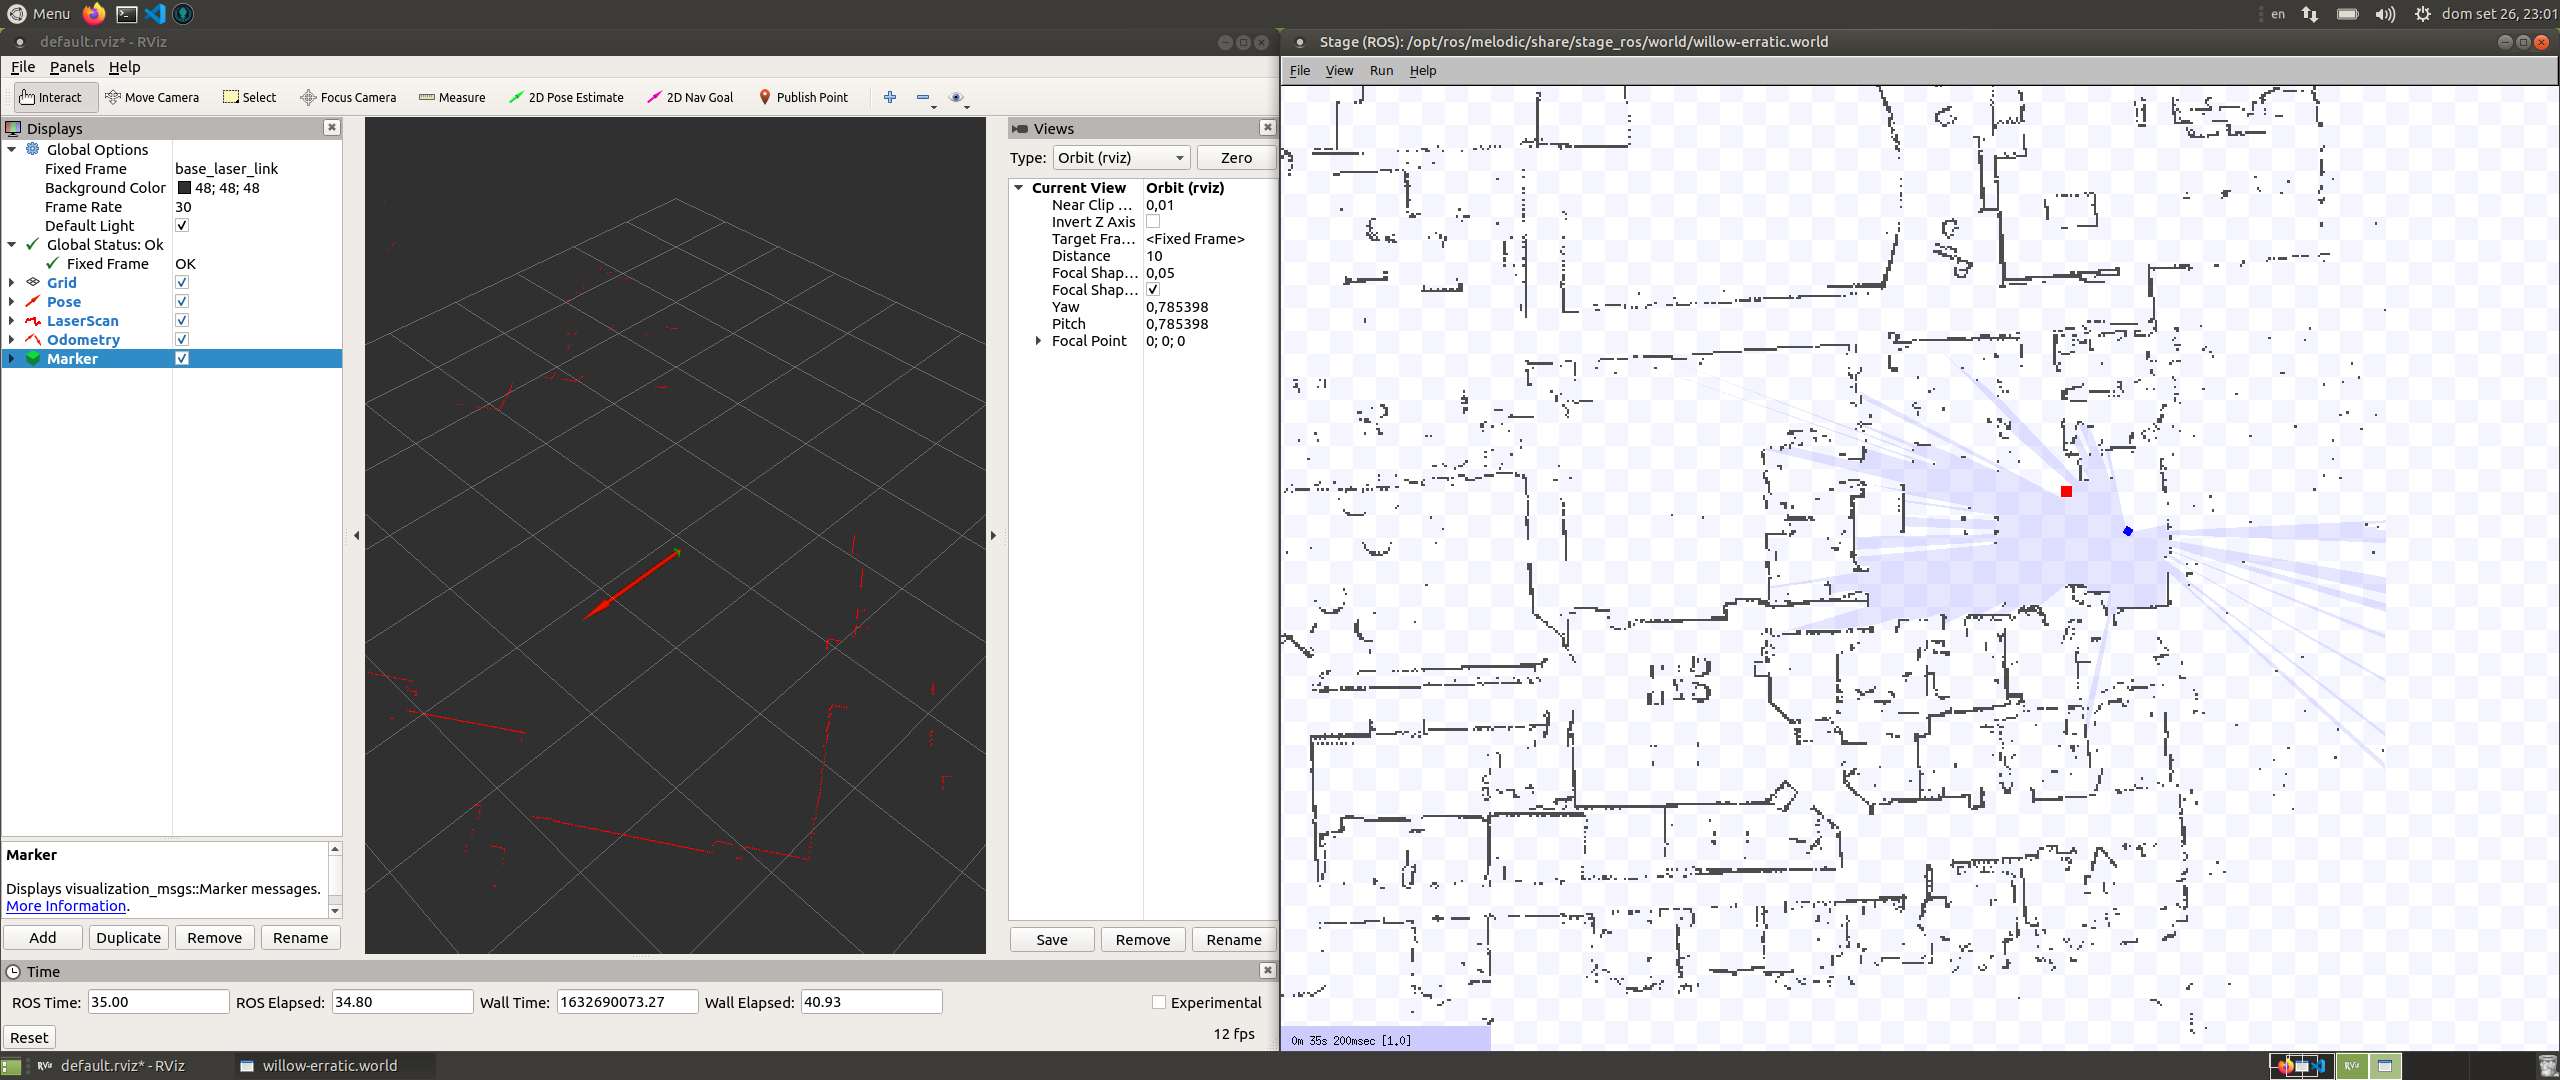
\includegraphics[width=13.5cm]{rviz_force1.png}
    \caption{Come è possibile notare, nel test analizzato si parte da una situazione in cui la risultante delle forze (rappresentata dalla freccia verde) è nulla, poiché il robot è abbastanza distante da qualsiasi ostacolo.}
    \label{fig:rviz_force1}
\end{figure}
\begin{figure}[htp]
    \centering
    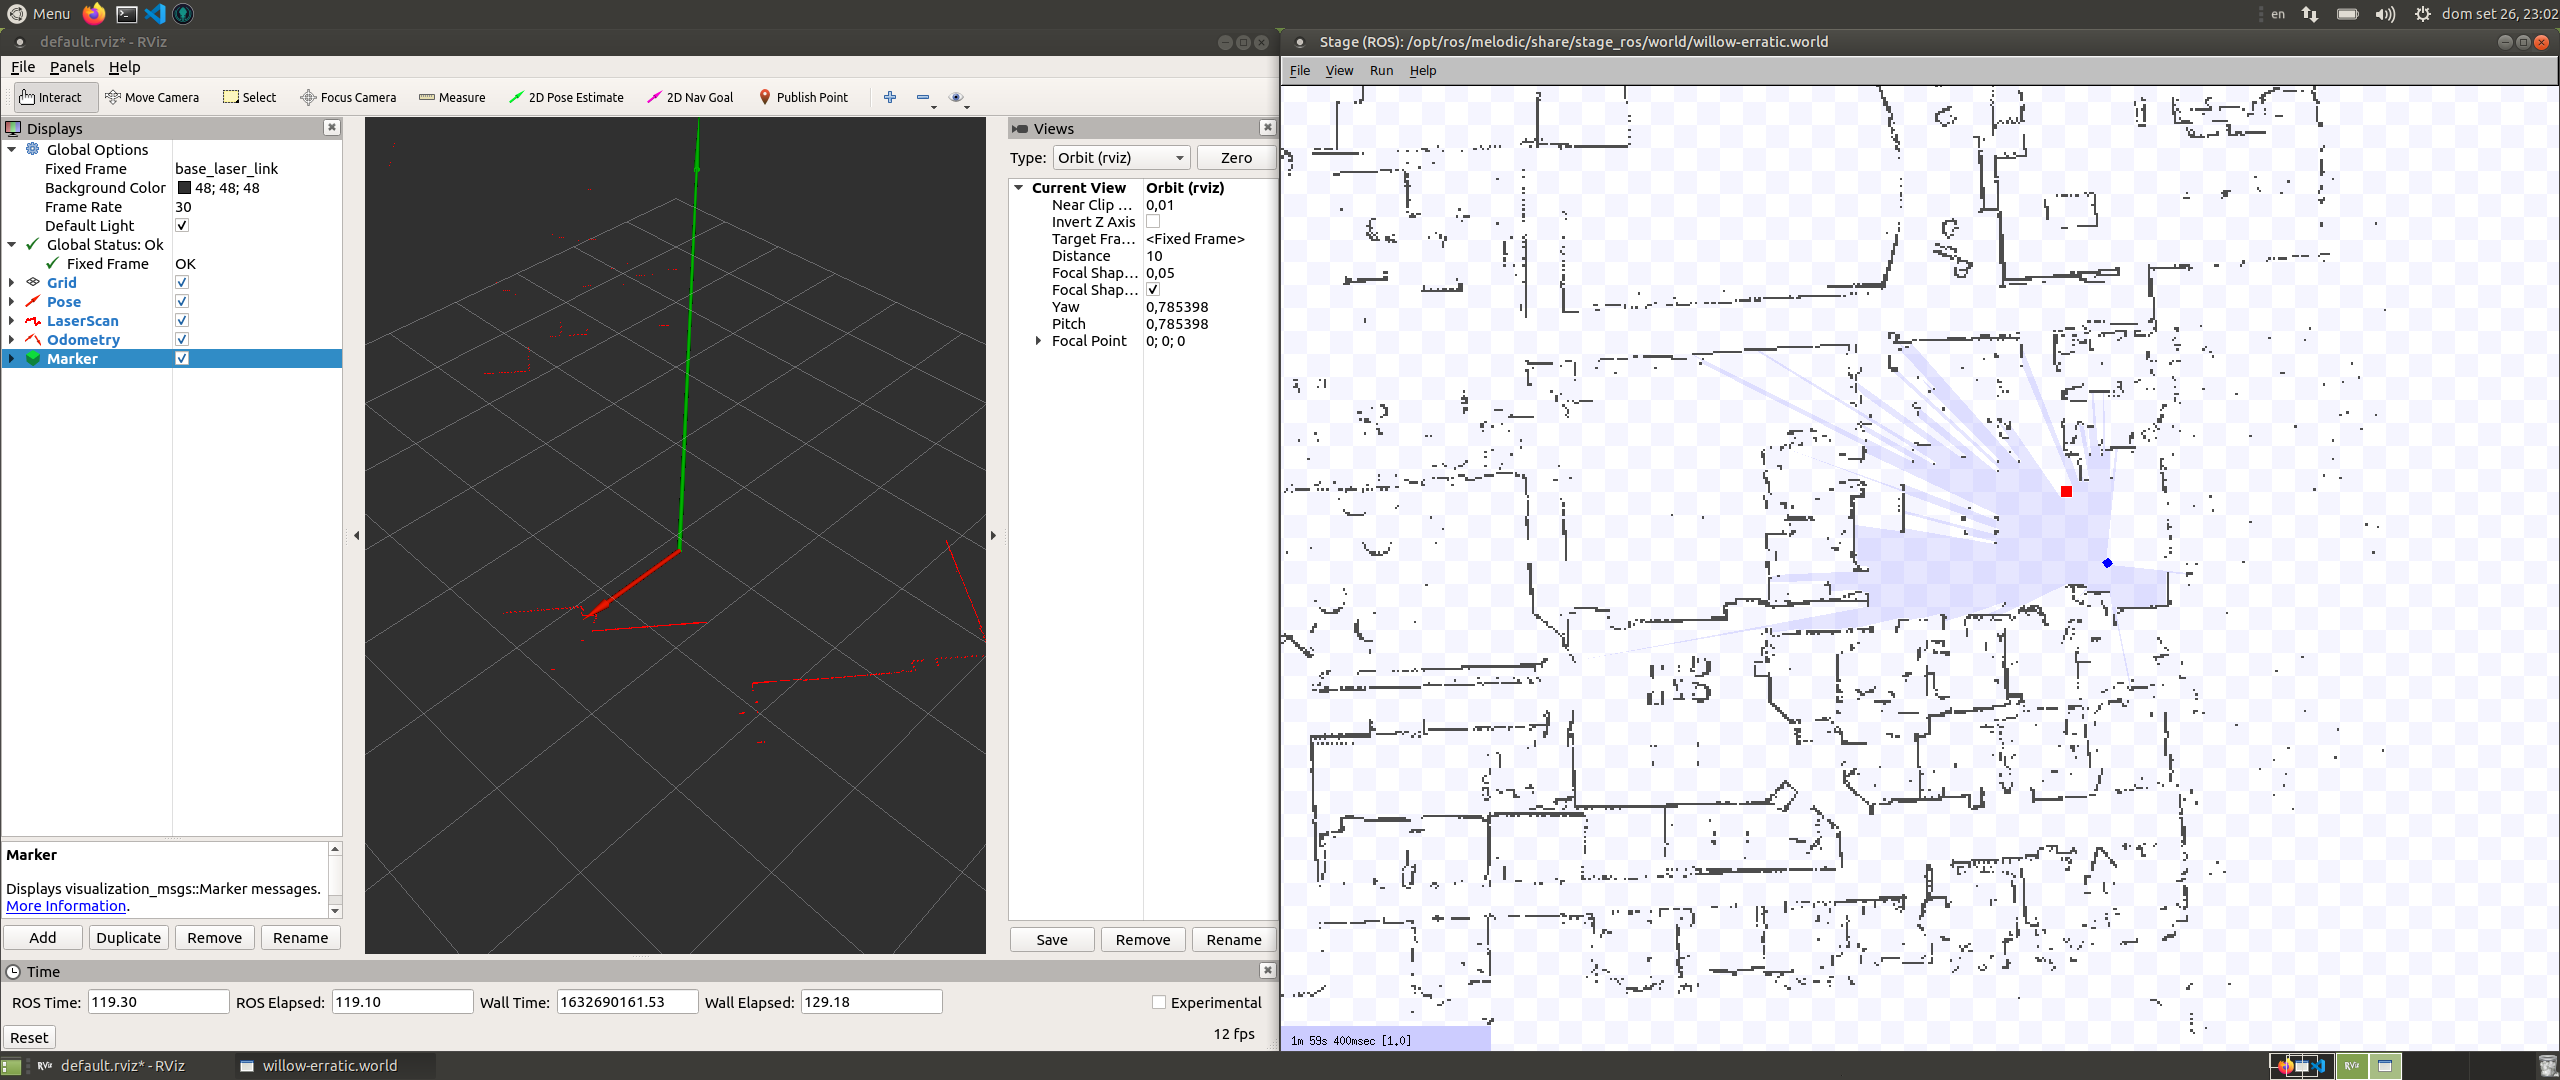
\includegraphics[width=13.5cm]{rviz_force2.png}
    \caption{Quando si prova ad avvicinare il robot a un ostacolo, la forza risultante aumenta notevolmente.}
    \label{fig:rviz_force2}
\end{figure}
\begin{figure}[htp]
    \centering
    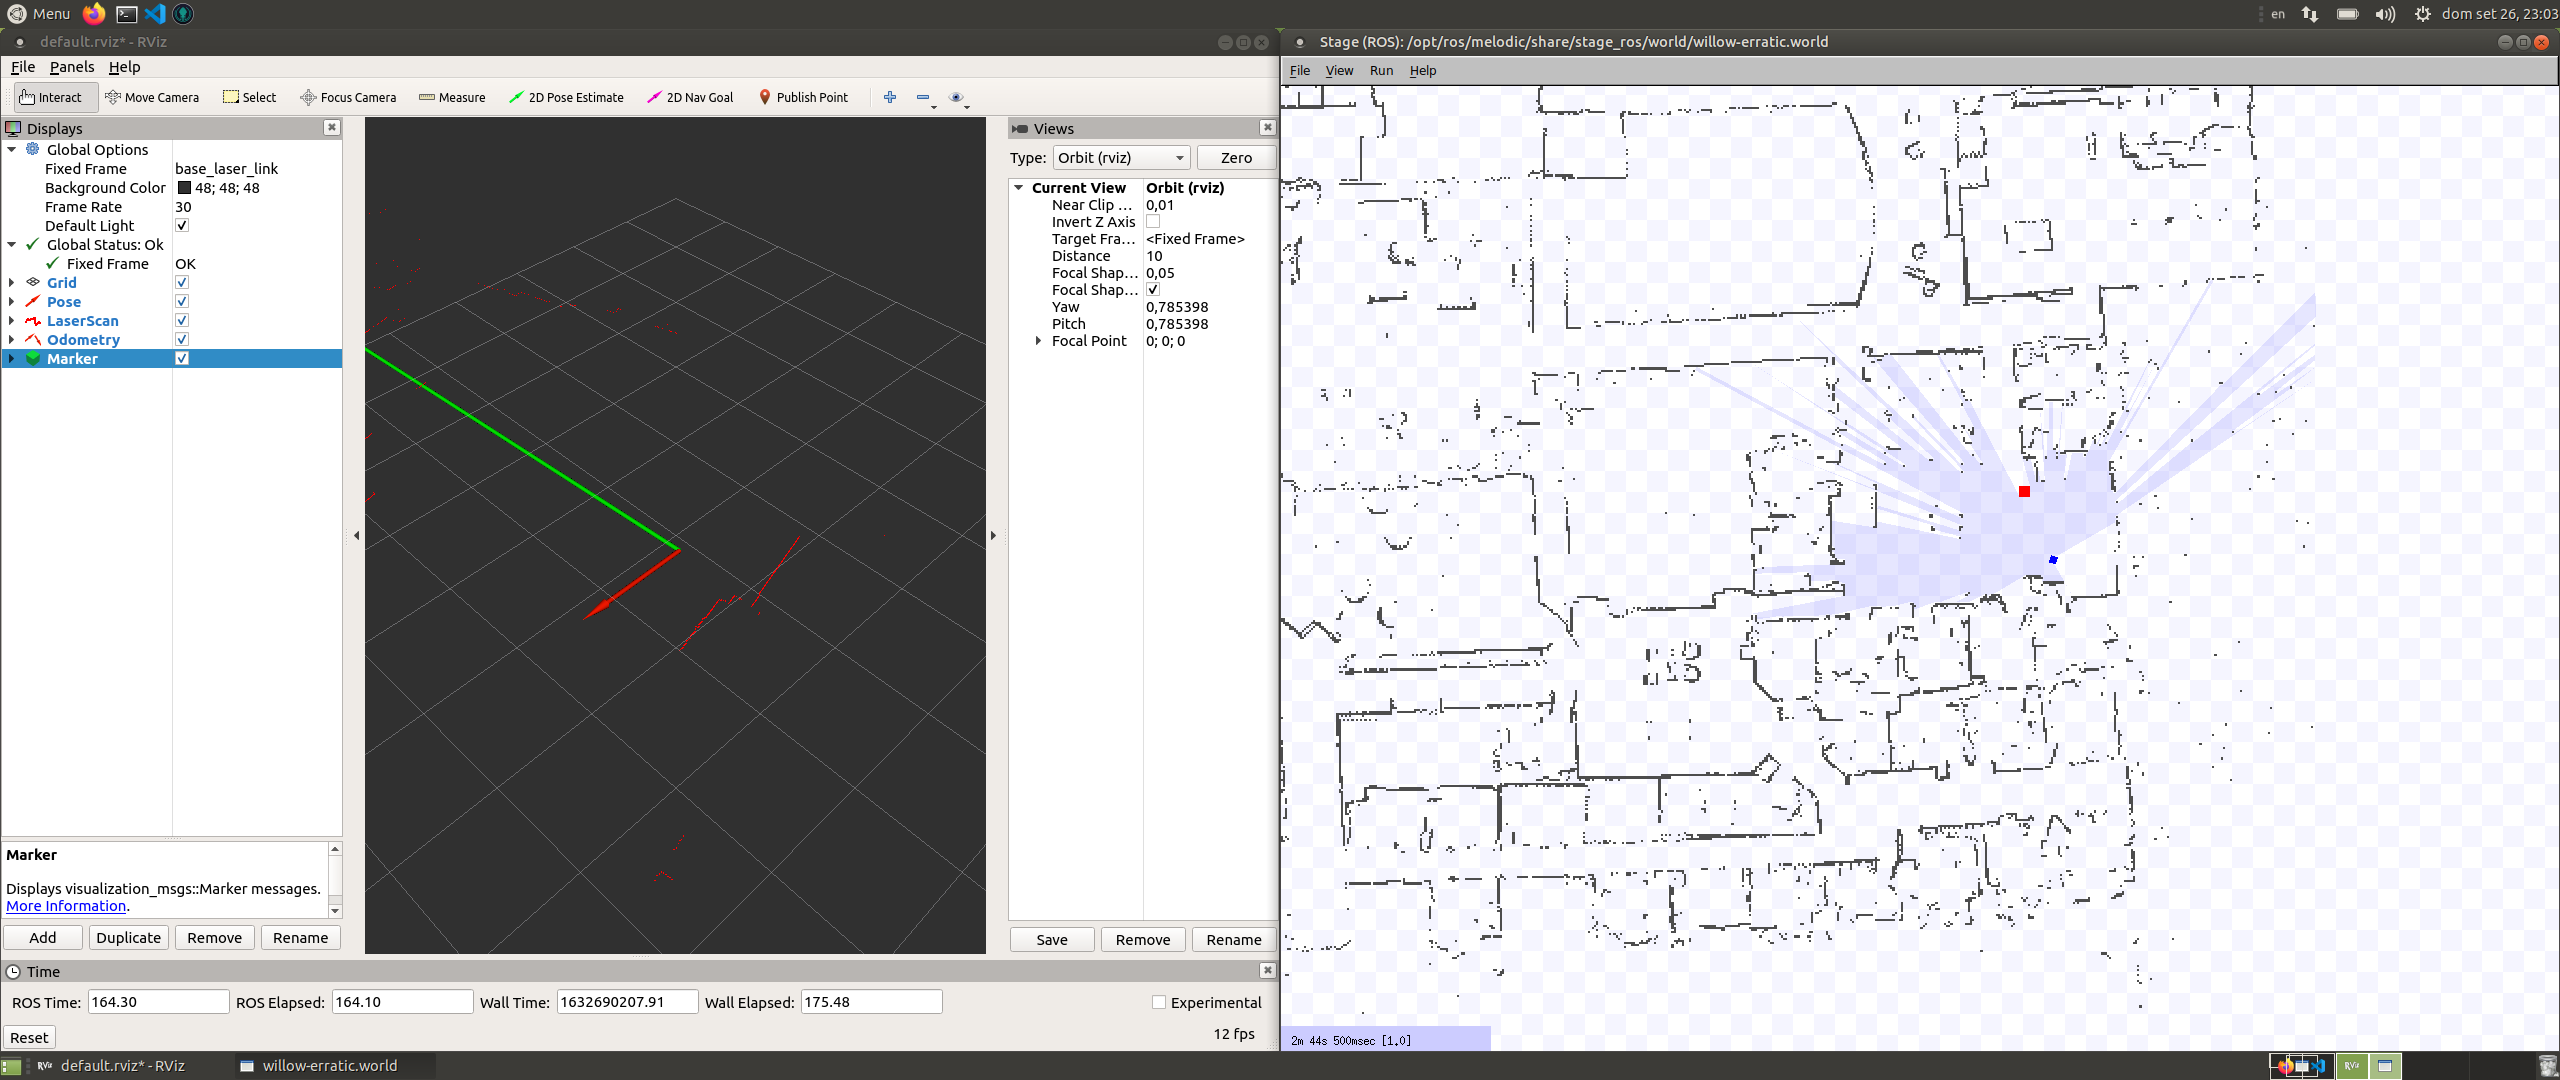
\includegraphics[width=13.5cm]{rviz_force3.png}
    \caption{La direzione del robot (rappresentata dalla freccia rossa) viene quindi corretta in base alla forza calcolata.}
    \label{fig:rviz_force3}
\end{figure}
\begin{figure}[htp]
    \centering
    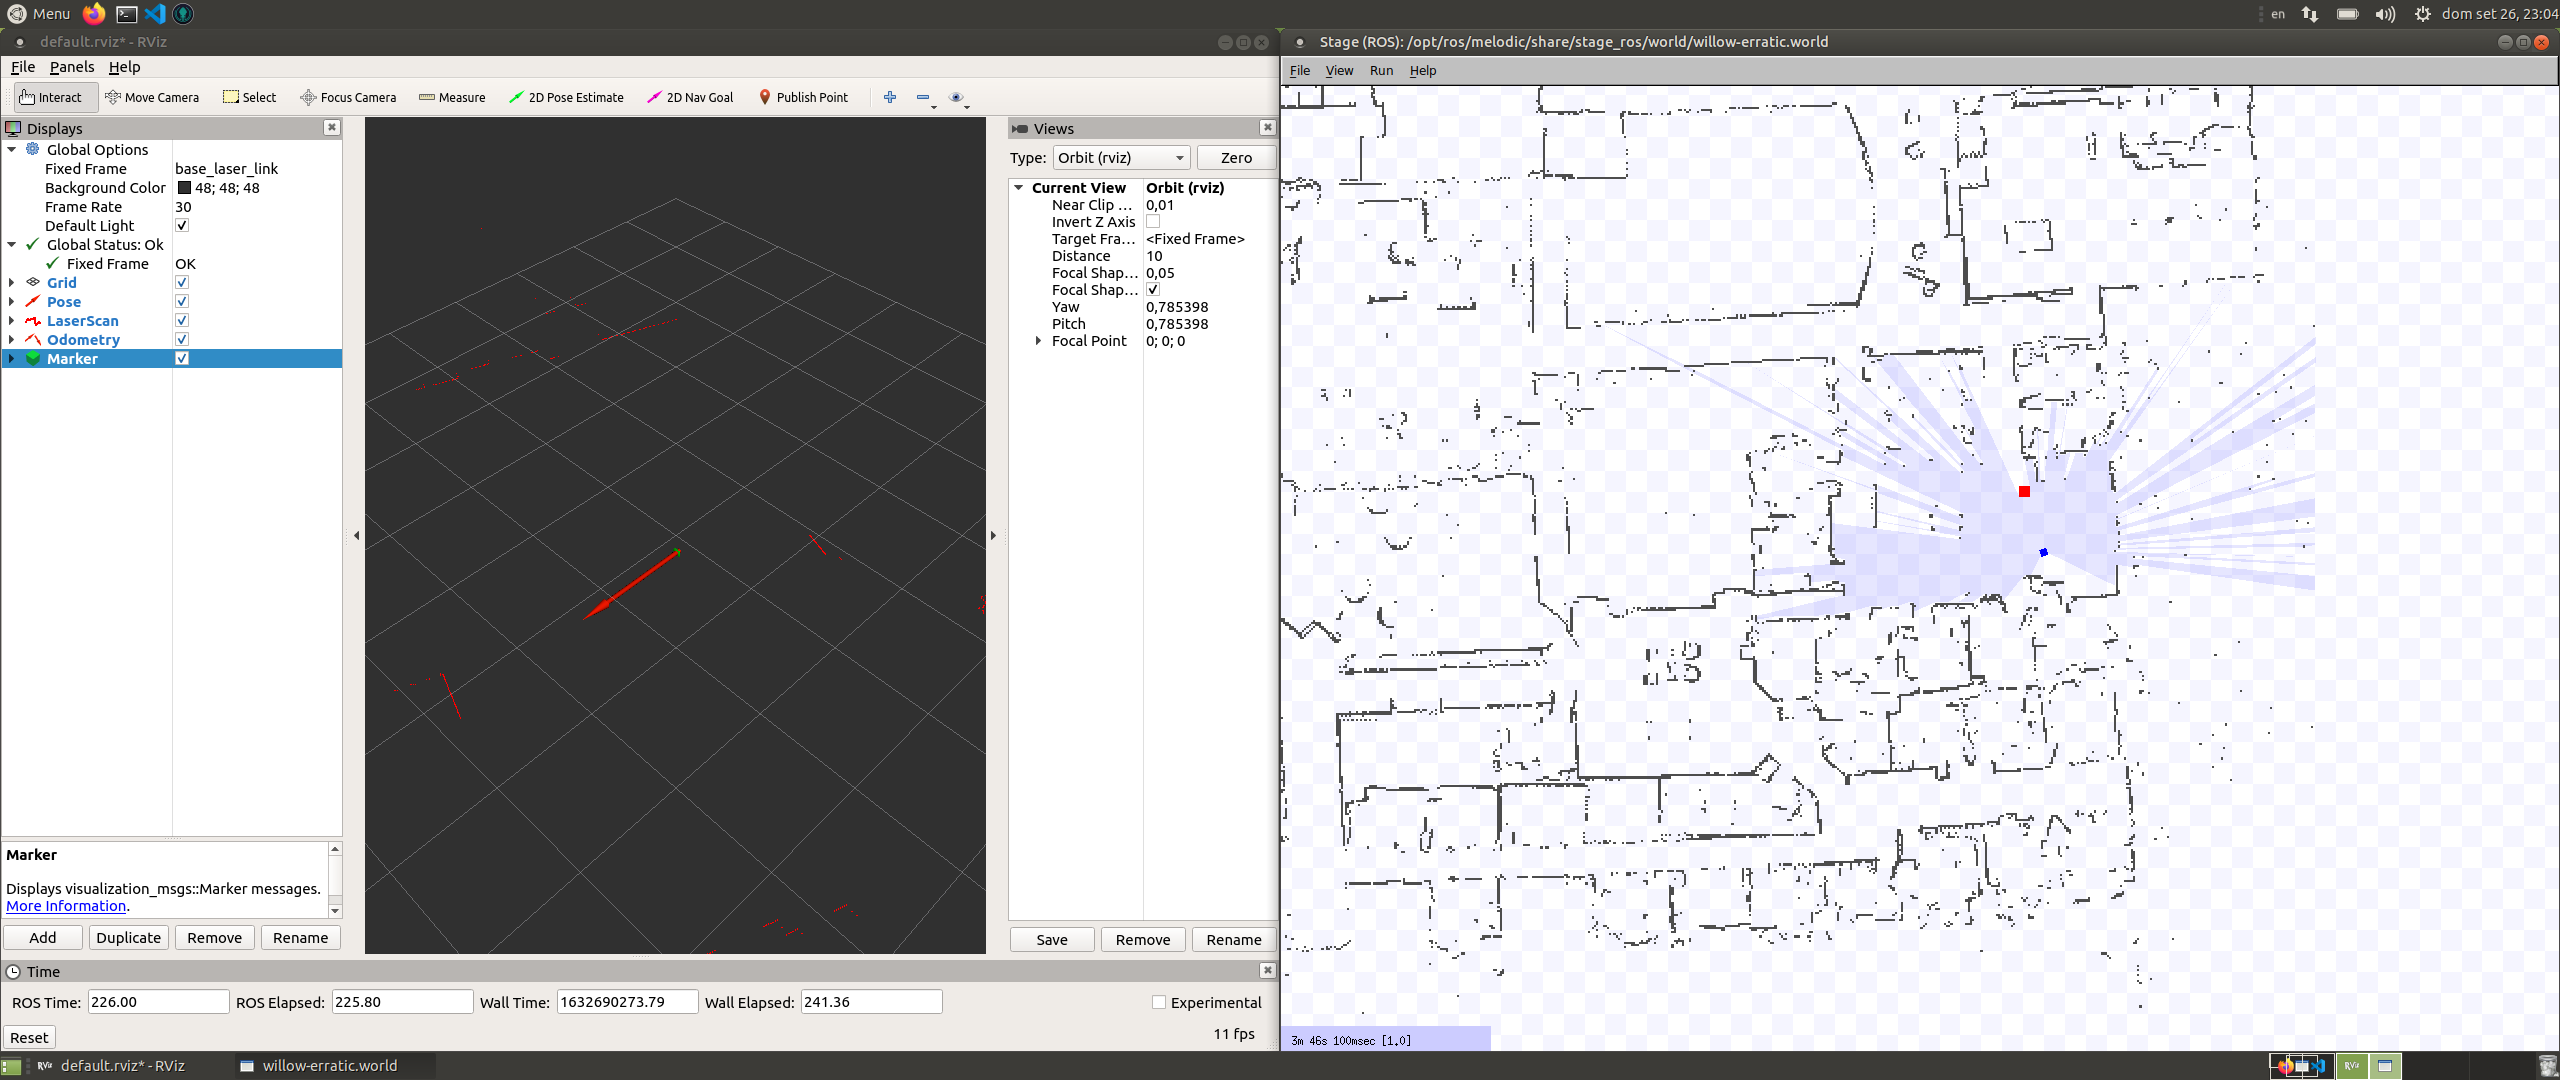
\includegraphics[width=13.5cm]{rviz_force4.png}
    \caption{Dopo le dovute correzioni, il robot viene portato in una zona in cui la presenza di ostacoli vicini è minore.}
    \label{fig:rviz_force4}
\end{figure}
\begin{figure}[htp]
    \centering
    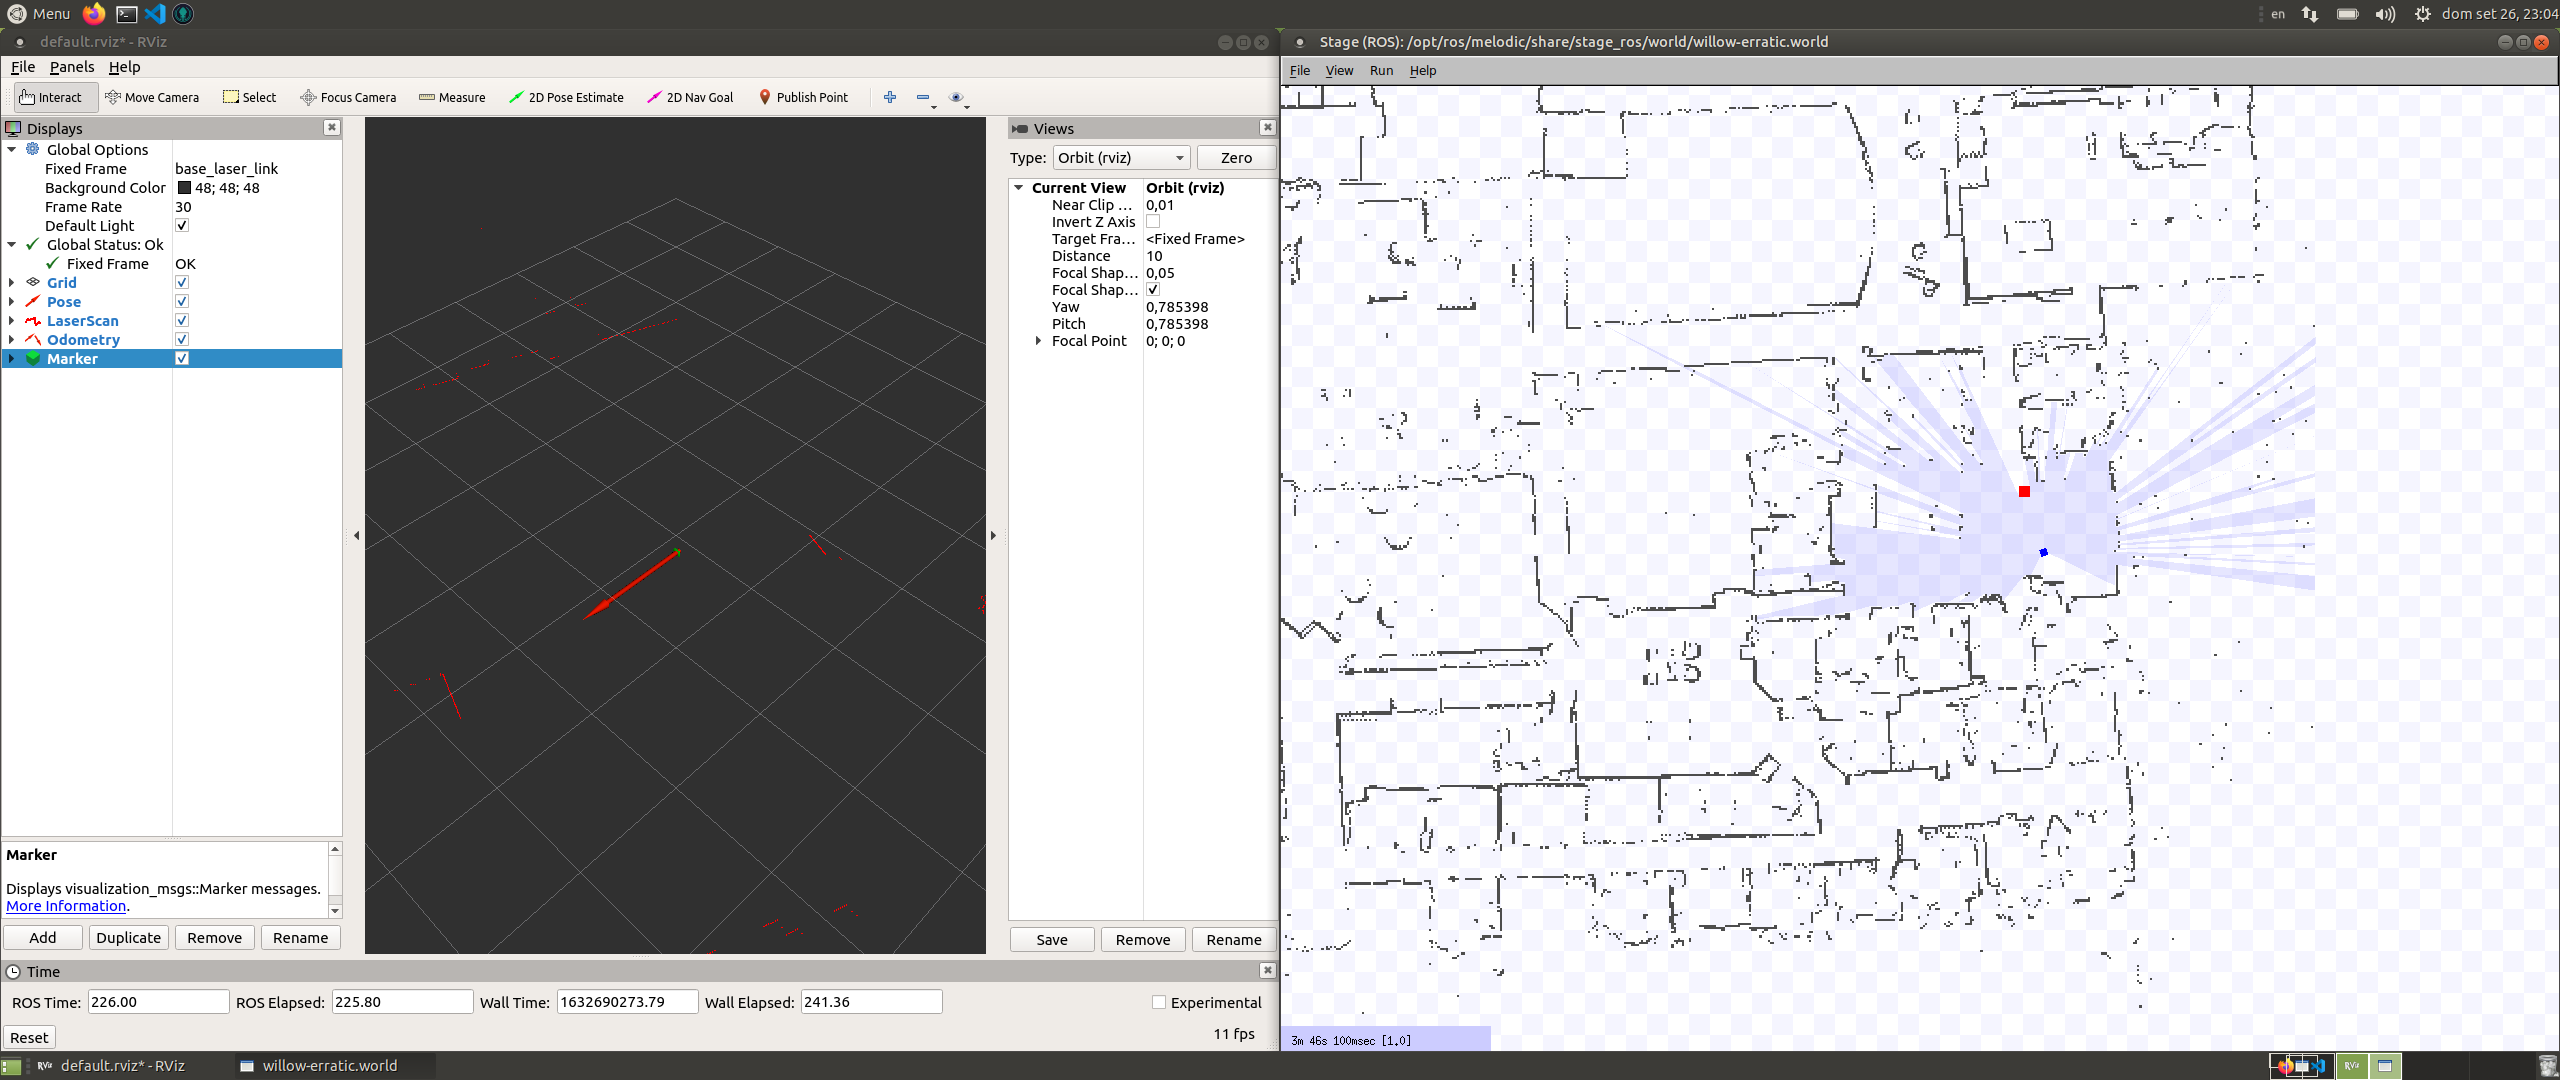
\includegraphics[width=13.5cm]{rviz_force5.png}
    \caption{Infine, il robot si trova nuovamente in una zona in cui il rischio di collisioni è minimo.}
    \label{fig:rviz_force5}
\end{figure}

\section{Analisi dei test e scelta dei parametri}
Durante la fase di test è stato necessario valutare i seguenti parametri:
\begin{description}
    \item[Soglia misurazioni scanner] Questo parametro serve a decidere quanto devono essere vicini gli ostacoli per costituire un possibile rischio di collisione.
    \item[Coefficiente velocità angolare] Questo parametro serve ad attenuare gli effetti della forza sulla velocità angolare del robot.
    \item[Coefficiente velocità lineare] Questo parametro serve ad attenuare gli effetti della forza sulla velocità lineare del robot.
\end{description}
Dopo aver svolto alcune osservazioni si è giunti ad una conclusione.

Per quanto riguarda il primo parametro, è stato scelto $1.25$ come distanza di soglia; infatti, è stato osservato che valori più bassi causano collisioni in alcune situazioni, mentre valori troppo alti limitano la libertà di manovra del robot, portandolo a volte a rimanere bloccato in un loop.

Per quanto riguarda il secondo ed il terzo parametro non è stato possibile trovare una combinazione di valori adeguata in quanto si è notato che valori troppo alti della velocità lineare di output potevano sempre portare a delle collisioni.
Si è optato quindi per limitare la velocità lineare di output a valori inferiori a $0.75$, scelta che rende quasi nulla la possibilità di collisione.
Con questo valore massimo è stato possibile scegliere pari a 1 il coefficiente per la velocità angolare, che non verrà quindi attenuata.

\chapter{Conclusioni}
Durante lo svolgimento di questo progetto è stato possibile capire l'importanza che possono ricoprire nella robotica gli algoritmi di local motion control.
Durante i test il robot è stato infatti messo in una condizione di totale assenza di informazioni riguardo alla mappa in cui era situato.
Tutti i calcoli fatti dal robot si basavano quindi solo sulle informazioni che potevano essere raccolte in tempo reale.
Questo evidenzia la capacità degli algoritmi di local motion control (come ad esempio quello dell'Artificial Potential Field, presentato in questo studio) di reagire prontamente a eventuali imprevisti.

È stato tuttavia messo in evidenza quanto sia importante la scelta dei parametri per il corretto funzionamento dell'algoritmo, che va effettuata a seguito di test e simulazioni.
Questi parametri potrebbero infatti cambiare in base all'applicazione che si deve fare dell'algoritmo.

Nonostante l'importanza di questo tipo di algoritmi, è stato possibile notare le loro limitazioni e la loro necessità di essere associato con algoritmi di global path planning (come ad esempio gli algoritmi A* e D*) e SLAM (Simultaneus Localization and Mapping), per avere una accuratezza e delle prestazioni migliori.

Oltre alla combinazione di algoritmi diversi, combinare le informazioni di più sensori rende più preciso il rilevamento degli ostacoli, diminuendo ancora di più i rischi.
A dimostrazione di ciò si può notare come le implementazioni presentate all'inizio facciano spesso uso di più sensori.
Per quanto riguarda le automobili vengono infatti usate le informazioni raccolte da radar, laser e camere, mentre per quanto riguarda l'esempio di SmartDect, ai tradizionali sistemi anticollisione sono state aggiunte maggiori informazioni provenienti dai dispositivi UWB.

\bibliographystyle{unsrt}
\bibliography{bibliografia.bib}

\end{document}